\documentclass[12pt,a4paper]{article}
\usepackage{amsmath,amsfonts,graphicx}
\topmargin=0pt
\headheight=0pt
\headsep=0pt
\textheight=750pt
\footskip=0pt
\voffset=-40pt
\textwidth=520pt
\marginparsep=0pt
\marginparwidth=0pt
\marginparpush=0pt
\oddsidemargin=0pt
\evensidemargin=0pt
\hoffset=-50pt
\newcommand{\ds}{\displaystyle}
\newcommand{\To}{\ \Rightarrow\ }
\newcommand{\pa}{\partial}
\newcommand{\Ol}{\overline}
\newcommand{\C}{\choose}
\newcommand{\m}[1]{\begin{bmatrix}#1\end{bmatrix}}
\newcommand{\ol}[1]{\begin{enumerate}#1\end{enumerate}}
\begin{document}
\noindent Intrinsic carrier densities(electrons and holes): 
$\ds n_i = BT^3 \exp(-\frac{E_G}{kT}) cm^{-6} = pn$\\
$\ds B = 1.08\cdot10^31K^{-3}\cdot cm^{-6}$ (Si).\\
Do\textbf{n}or: \textbf{n}-type $\To$ Acce\textbf{p}ter: \textbf{p}-type\\
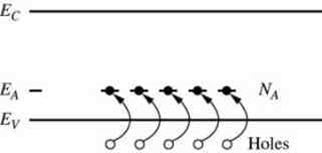
\includegraphics[scale=.5]{acceptor.png}
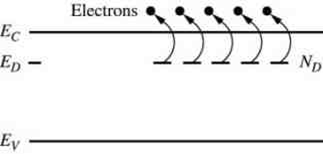
\includegraphics[scale=.5]{donor.png}
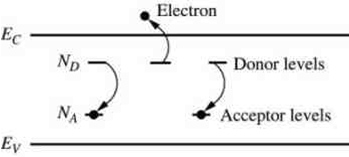
\includegraphics[scale=.5]{band.png}\\
Electron mobility($\mu_n$), hole mobility($\mu_p$)\\
Conductivity: $\ds\sigma = q(\mu_nn+\mu_pp)$,
Resistivity: $\ds\rho = \frac{1}{\sigma}$\\
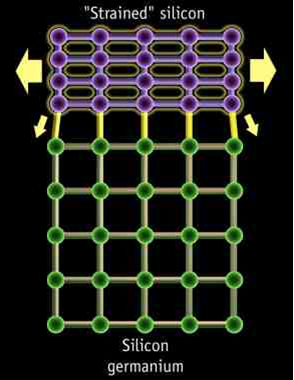
\includegraphics[scale=.5]{strained_si.png}\\
Strained Silicon:\ol{
    \item Strained Silicon increases transistor drive current which improves switching speed by making current flow more smoothly. 
    \item Has negligible effect on manufacturing cost.
}
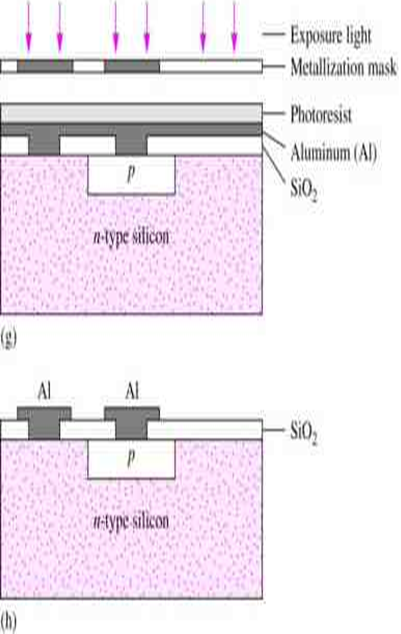
\includegraphics[scale=.5]{icfab.png}
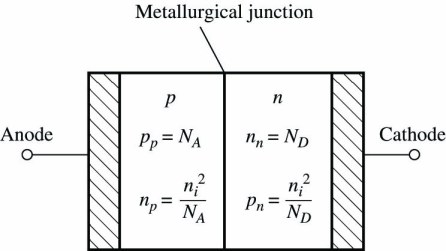
\includegraphics[scale=.5]{pn.png}\\
$\ds\Phi_j=V_T\ln\left(\frac{N_AN_D}{n_i^2}\right),\ w_{do}=(x_n+x_p)
=\sqrt{\frac{2\epsilon_s}{q}\left(\frac{1}{N_A}+\frac{1}{N_D}\right)\Phi_j},\ 
E_{MAX}=\frac{2\Phi_j}{w_{do}}\ \ (\ln10\approx2.3)\\
\epsilon_s=11.7\epsilon_o,\ \epsilon_o=8.85\cdot10^{-14},\ 
q=1.60\cdot10^{-19}$(silicon)\\
$\ds i_D=I_S\left[\exp\left(\frac{qv_D}{nkT}\right)-1\right]
=I_S\left[\exp\left(\frac{qv_D}{nV_T}\right)-1\right],\ V_T=0.025$ V(room temp.)
\\\\
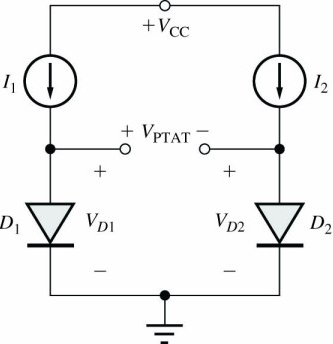
\includegraphics[scale=.5]{ptat0.png}
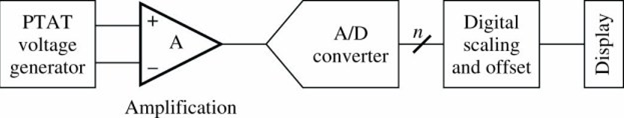
\includegraphics[scale=.5]{ptat1.png}\\
PTAT Voltage and Electronic Thermometry:\ol{
    \item The well-defined temperature dependence of the diode voltage is used as the basis for most digital themometers.
    \item $\ds V_{PTAT}=V_{D1}-V_{D2}
    =V_T\ln\frac{I_{D1}}{I_S}-V_T\ln\frac{I_{D2}}{I_S}
    =V_T\ln\frac{I_{D1}}{I_{D2}}=\frac{KT}{q}\ln\frac{I_{D1}}{I_{D2}}$
    \item By using two diode, the temperature dependence of Is has been eliminated from the equation.
}
Reverse bias saturation current: $\ds I_S=I_{S0}\sqrt{1+\frac{v_R}{\Phi_j}}\\$
Rectfier Circuits: 
$\ds v_P=\sqrt{2}v_{rms},\ v_0=v_P-v_{on},\ 
C=\frac{V_0T}{V_rR},\ PIV=2V_P,\ I_{SC}=\omega CV_p=2\pi fCV_p,\\
\Delta T=\frac{1}{\omega}\sqrt{\frac{2V_r}{V_p}},\
I_P=I_{dc}\frac{2T}{\Delta T}
=\frac{V_0}{R}\frac{2T}{\Delta T},\ P_D\approx V_{on}I_{dc}$
\\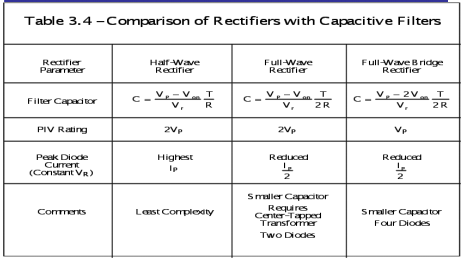
\includegraphics[scale=.75]{cmp.png}
\end{document}
